\documentclass[a4paper]{article}\usepackage[]{graphicx}\usepackage[]{xcolor}
% maxwidth is the original width if it is less than linewidth
% otherwise use linewidth (to make sure the graphics do not exceed the margin)
\makeatletter
\def\maxwidth{ %
  \ifdim\Gin@nat@width>\linewidth
    \linewidth
  \else
    \Gin@nat@width
  \fi
}
\makeatother

\definecolor{fgcolor}{rgb}{0.345, 0.345, 0.345}
\newcommand{\hlnum}[1]{\textcolor[rgb]{0.686,0.059,0.569}{#1}}%
\newcommand{\hlstr}[1]{\textcolor[rgb]{0.192,0.494,0.8}{#1}}%
\newcommand{\hlcom}[1]{\textcolor[rgb]{0.678,0.584,0.686}{\textit{#1}}}%
\newcommand{\hlopt}[1]{\textcolor[rgb]{0,0,0}{#1}}%
\newcommand{\hlstd}[1]{\textcolor[rgb]{0.345,0.345,0.345}{#1}}%
\newcommand{\hlkwa}[1]{\textcolor[rgb]{0.161,0.373,0.58}{\textbf{#1}}}%
\newcommand{\hlkwb}[1]{\textcolor[rgb]{0.69,0.353,0.396}{#1}}%
\newcommand{\hlkwc}[1]{\textcolor[rgb]{0.333,0.667,0.333}{#1}}%
\newcommand{\hlkwd}[1]{\textcolor[rgb]{0.737,0.353,0.396}{\textbf{#1}}}%
\let\hlipl\hlkwb

\usepackage{framed}
\makeatletter
\newenvironment{kframe}{%
 \def\at@end@of@kframe{}%
 \ifinner\ifhmode%
  \def\at@end@of@kframe{\end{minipage}}%
  \begin{minipage}{\columnwidth}%
 \fi\fi%
 \def\FrameCommand##1{\hskip\@totalleftmargin \hskip-\fboxsep
 \colorbox{shadecolor}{##1}\hskip-\fboxsep
     % There is no \\@totalrightmargin, so:
     \hskip-\linewidth \hskip-\@totalleftmargin \hskip\columnwidth}%
 \MakeFramed {\advance\hsize-\width
   \@totalleftmargin\z@ \linewidth\hsize
   \@setminipage}}%
 {\par\unskip\endMakeFramed%
 \at@end@of@kframe}
\makeatother

\definecolor{shadecolor}{rgb}{.97, .97, .97}
\definecolor{messagecolor}{rgb}{0, 0, 0}
\definecolor{warningcolor}{rgb}{1, 0, 1}
\definecolor{errorcolor}{rgb}{1, 0, 0}
\newenvironment{knitrout}{}{} % an empty environment to be redefined in TeX

\usepackage{alltt}

% ----- dependencies
\usepackage{lmodern} % improve font quality
\usepackage{hyperref} % url links
\usepackage{graphicx} % insert image
\usepackage{tabularx} % default tabular breaks inside mini-page
\usepackage{enumitem} % customize itemize elements
\usepackage{xcolor} % color text
\usepackage{fp} % floating point arithmetic
\usepackage{fontawesome5} % icons
\usepackage{tikz} % svgs
\usepackage{adjustbox} % adjusting image position
\usepackage[most]{tcolorbox} % badges
\usepackage{listings}
\lstset{basicstyle=\ttfamily,
  showstringspaces=false,
  commentstyle=\color{red},
  keywordstyle=\color{blue}
}

% ----- configure: font type
\renewcommand{\familydefault}{\rmdefault} % choose: \rmdefault, \ttdefault, \sfdefault
\urlstyle{same}

% ----- configure: font size
\newcommand{\fontSize}{9pt}
\usepackage[fontsize=\fontSize]{scrextend}

% ----- configure: page margin
\newcommand{\margin}{20mm}
\usepackage[margin=0px, top=\margin, bottom=\margin, left=\margin, right=\margin]{geometry}
\setlength\parindent{0pt}
\IfFileExists{upquote.sty}{\usepackage{upquote}}{}
\begin{document}

% header
\begin{center}
  \LARGE{\textbf{sweave demo}}
\end{center}

this file is a demo for the sweave package that allows to embed R code inside latex documents.

\section{how to run this}

here's how to get the output of this file:

\begin{lstlisting}[language=bash]
#!/bin/bash
rscript -e "Sweave('file.rnw')" # get the .tex file
rscript -e "Stangle('file.rnw')" # get the .R file
\end{lstlisting}

but be careful, as you'll most likely miss the \texttt{Sweave.sty} dependency when compiling the \texttt{.tex} file.

\section{the code}

here's our R code block that's embedded inside the latex document.

% show results
\begin{knitrout}
\definecolor{shadecolor}{rgb}{0.969, 0.969, 0.969}\color{fgcolor}\begin{kframe}
\begin{alltt}
\hlstd{x} \hlkwb{<-} \hlnum{1}\hlopt{:}\hlnum{10}
\hlstd{y} \hlkwb{<-} \hlstd{x}\hlopt{^}\hlnum{2}

\hlkwd{plot}\hlstd{(x, y)}
\end{alltt}
\end{kframe}

{\centering 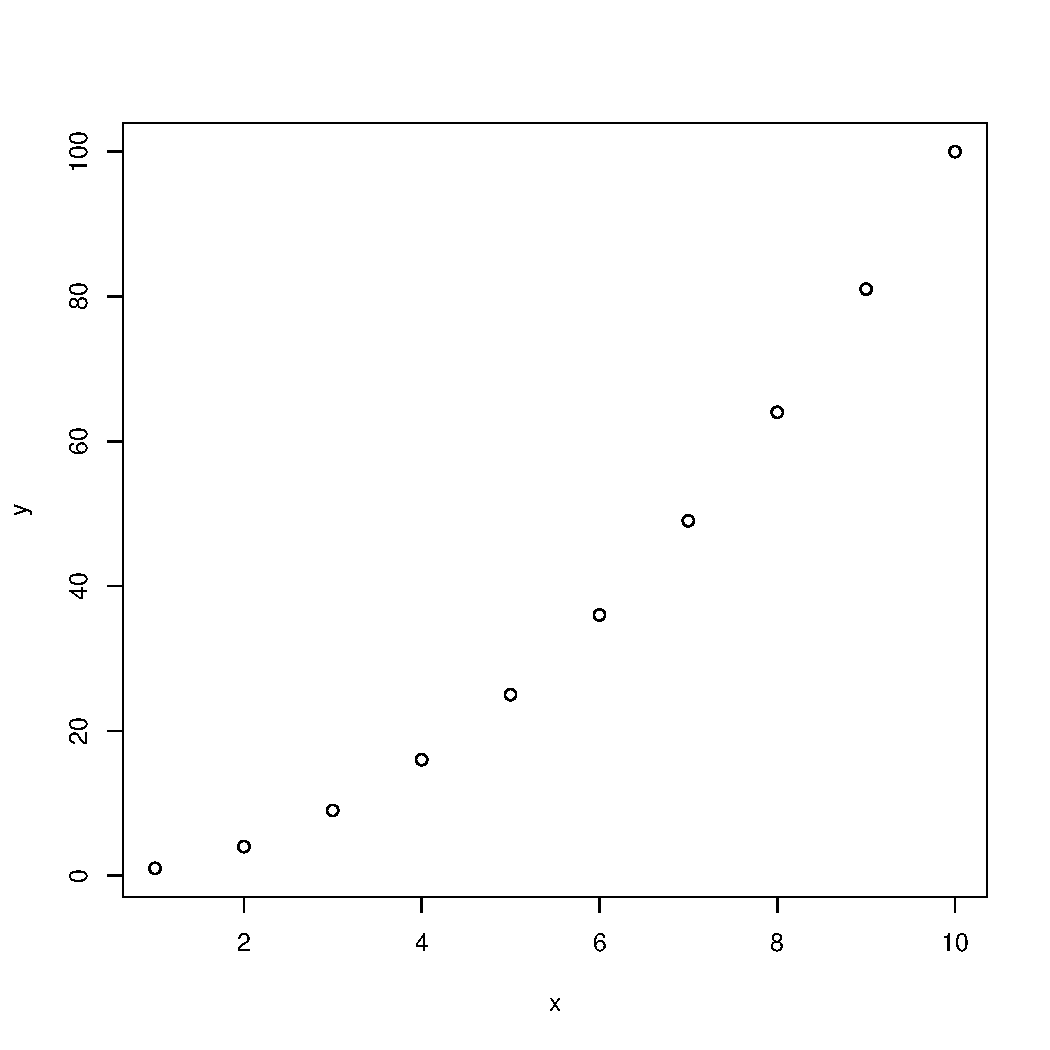
\includegraphics[width=3in]{figure/demo-1} 

}


\begin{kframe}\begin{alltt}
\hlkwd{print}\hlstd{(x)}
\end{alltt}
\begin{verbatim}
##  [1]  1  2  3  4  5  6  7  8  9 10
\end{verbatim}
\begin{alltt}
\hlkwd{print}\hlstd{(y)}
\end{alltt}
\begin{verbatim}
##  [1]   1   4   9  16  25  36  49  64  81 100
\end{verbatim}
\end{kframe}
\end{knitrout}

\section{the config}

when embedding code blocks, here are some possible options for the sweave package:

\begin{itemize}
  \item \texttt{echo} = show the code block
  \item \texttt{eval} = evaluate the code block
  \item \texttt{results} = show the results
  \item \texttt{fig} = show the figures
  \item \texttt{eps} = export the figures as eps
\end{itemize}

\end{document}
